\documentclass{llncs}
\usepackage{graphicx}
\graphicspath{ {images/} }


\title{\textbf{Random Forest vs Logistic Regression for Binary Classification}}
\author{Kaitlin Kirasich, Trace Smith, and Bivin Sadler, PhD$^1$}
\institute{$^1$Master of Science in Data Science \\ Southern Methodist University \\ Dallas, Texas USA \\
\email{kkirasich@.smu.edu,traces@smu.edu,bsadler@smu.edu}}

\begin{document}
\maketitle

\begin{abstract} 
Selecting a learning algorithm to implement for a particular application on the basis of performance still remains an ad-hoc process using fundamental benchmarks such as evaluating a classifier’s overall loss function, area under the curve (AUC) score, specificity, and sensitivity values. This work is aimed at addressing the difficulty of model selection by evaluating the overall classification performance between random forest and logistic regression for datasets comprised of various underlying structures. A model evaluation tool was developed in R for simulating a variety of dataset characteristics in order to evaluate performance metrics such as true positive rate, false positive rate, and accuracy under specific conditions. Our findings indicate that when increasing the variance in the explanatory and noise variables, logistic regression consistently performed with a higher overall accuracy as compared to random forest.  However, the true positive rate for random forest was higher than logistic regression and yielded a higher false positive rate. In all cases a paired two sample t-test indicates there is enough evidence to suggest the false positive rate for random forest is statistically different than logistic regression. The model evaluation application developed in this work is a foundation for answering other intruiguing questions related to model performance under various treaments. 

\end{abstract}


\section{Introduction}

Datasets consist of various shapes and compositions, which poses the question, what data characteristics result in one machine learning algroithm outperforming others. Both quantitative and qualitative, data can be a combination of categorical and numerical multivariates that can range from a variety of entities. When it comes to model selection, this is a constant challenge data scientist are often faced with. Training and evaluating multiple machine learning models for a given use case can be an expensive task computationally and time consuming. The analysis presented in this work is to provide insight into the relative performance of a learning algorithm conditioned on the particular characteristics of a dataset. To do so, random forest and logistic regression are the two models that will be analyzed for comparing binary classification (y = {0,1}) performances with differing dataset structures. Both classifiers have been widely implemented in various domains and their successes have been well documneted. However, the particular characteristics of a dataset that make one model outperform the other is unknown as most published work compares overall performance between the two models for a single dataset. The objective of this study is to develop a statisitcal tool to directly observe the accuracy of each model by averaging the accuracy rate of 1000 random generations of assorted multivariate datasets. Classification metrics, such as accuracy, area under the curve, true positive rate, false positive rate, and precision are examined for model performance. Finally a pairwise two-sample t-test is conducted at the end of each simulation case study in order to provide statistical quantification as to whether a difference in model performance is conclusive enough to state the difference is significant or if the observed difference is by random chance. 


Characteristics of a dataset can be comprised of missing values, outlier, highly correlated variables, concave or convex shapes, or subsets of the data that can be represented as clusters. Complex datasets that are not linearly seperable, or in other words, where a linear hyperplane splits the data into two halves such that the model poorly predicts the class label of the respected observation (Figure 1). One approach to infering underlying complexities of high-dimensional dataset is Topological Data Analysis (e.g. TDA), an evolving method that utilizes topological and geometric tools to identify relevant features in the data. Robust to noisy and incomplete datasets, TDA can be described as method that helps identify structures like clusters or other hidden shapes that can provide a more accurate representation of the dataset (Chazal et al, 2017). Models can then be trained on the new representaiton of the data that has been reconstructed, which has shown promising results.While TDA looks at the proximity of data points and connectivity that can be mapped to a 1-dimensional plane for representing the shape of the data (Munch,2017), our analysis is aimed at creating various complexities in the data and evaluating model performance on the raw structure in a multidimensional space. For instance, altering the variance in the explanatory and noise variables, changing the number of observations, and varying the number of continuous features included in a multivariate dataset was considered. Investigation into why models like logistic regression or random forest perform differently for simple and complex data characteristics was the motivation behind this work.


Performance of machine learning classifiers can yield varying results depending on the shape and structure of the data. The data examined in this work is only for continuous variables that have a gaussian distribution. However, more complex structures can exists like the toy dataset shown below in Figure 1 and Figure 2 which consists of concave and convex shape. As illustrated below in Figure 1 and Figure 2, both random forest and logistic regression nearly establishes an identical decision boundary for the left-hand side dataset. Alternatively, logistic regression underperforms random forest and yields a higher missclassification rate, which raises a profounding questions as to which data characteristics consitutes one model acheiving an overall better classification score. It should be noted this work only investigates random forest and logistic regression, however generalizaiton of the current applicaiton can be adapted to other linear and nonlinear models. 

\begin{figure}
\centering
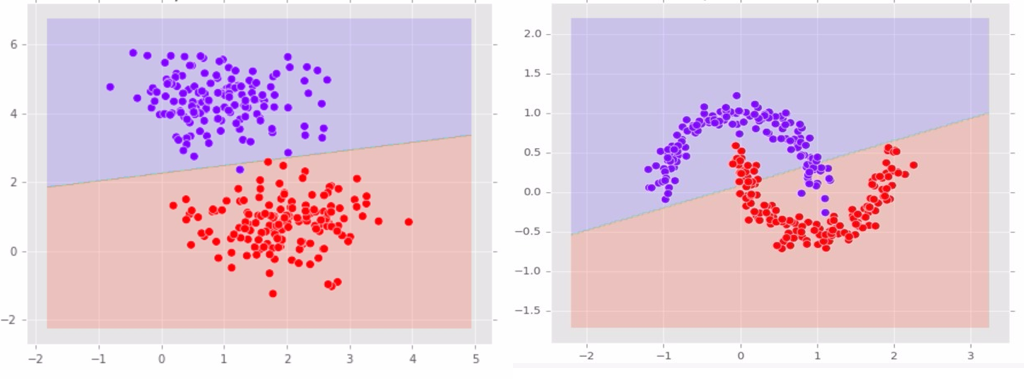
\includegraphics[width=0.9\textwidth]{decisionboundary.png}
\caption{Logistic Regression Decision Boundary}
\end{figure}

\begin{figure}
\centering
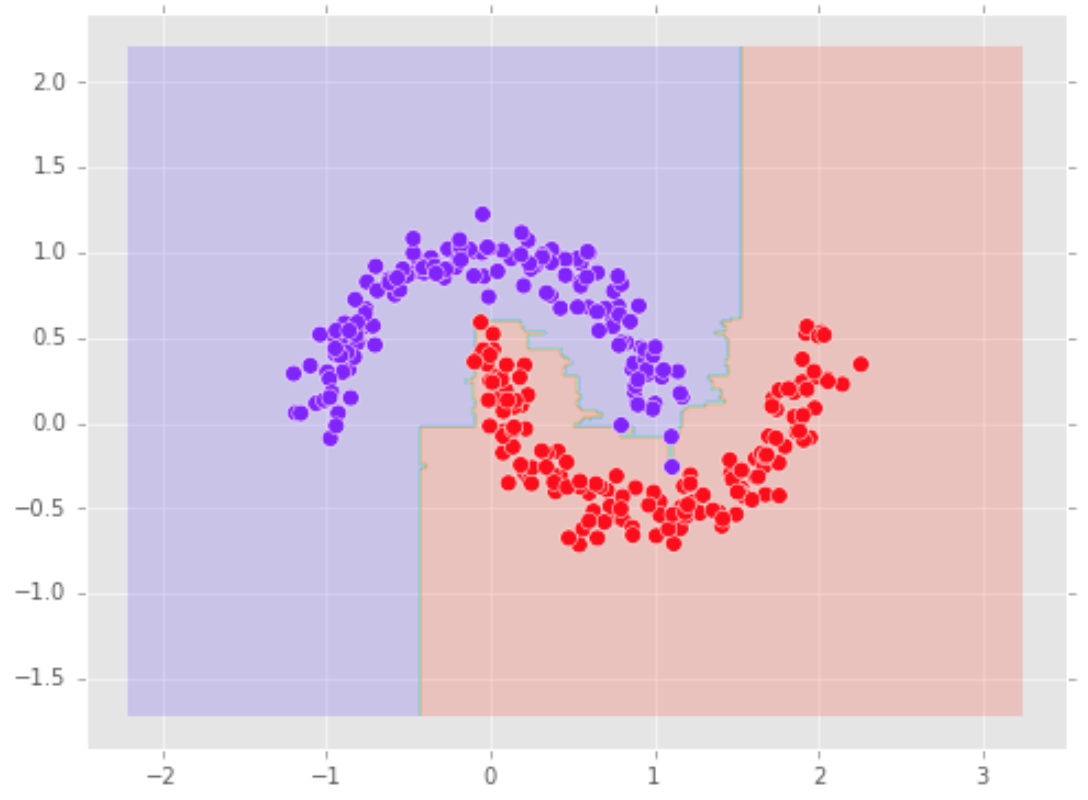
\includegraphics[width=0.9\textwidth]{decisionboundary2.png}
\caption{Random Forest (n-Trees = 100) Decision Boundary}
\end{figure}


Numerous studies have been published that compare random forest and logistic regression algorithms however, most research experiments consisted of either a single dataset or multiple datasets from the same source. In these scenarios, sometimes logistic regression performed better while in other cases random forest performed better. For example, one experiment used several neuropsychological tests to predict dementia stated that with respect to specificity and overall classification accuracy, random forests and linear discriminant analysis rank first among all the classifiers including logistic regression (Guerreiro, 2011). Contrastingly, in another article analyzing Twitter tweets surrounding the 2016 United States election, it was found that when PCA is applied to tweets, logistic regression provides better results than random forest (Begenilmis, 2017). The type of data and data sources used in the studies above are drastically different from each other and each algorithm performs differently due to the type of data it was using to try to classify. Our project aims to provide a method to evaluate random forest and logistic regression models for a variety of data conditions.

Criteria for identifying significant input features in a model varies between domains and datasets at hand. Automated feature selection has widely been studied, ranging from computer vision, classification, and regression types of problems. Zoran et al proposed a purposeful selection algorithm that automates feature selection by iteratively refitting the model by either adding or removing variables to verify if the model contains statistically significant predictors with a maximum p-value of 0.25 (Zoran, 2008). Traditionally, the significance threshold is 0.05; because there is only a 5\% chance of a Type I error, variables of importance could be misclassified. In this simulation study, the selection method evaluates significance at the 0.10 level and if the parameter estimate value alters 20\% compared to the full model, then there is evidence the excluded variable was of importance and is therefore added back to the model (Zoran, 2008). The novel method was applied on two different simulated datasets and was compared with stepwise, forward, and backward selection as a benchmark for the conclusion.  Logistic regression was the model of choice for the two simulation experiments performed by Zoran et al, consisting of six total explanatory variables and six different sample sizes. The first study consisted of only three significant variables of equal parameter estimates and three non-significant predictors. Secondly, the simulation was altered slightly to contain two significant variables, one confounder which is dependent on X1, and three non-significant variables with parameter estimate of zero, respectively. For both simulation cases, the average retention rate for 1000 iterations correctly identified variables increased with respect to an increase in sample size (Zoran, 2008).

\section{Data Set}

To conduct the statistical analysis, an interactive web application was developed using RShiny which allows end users to rapidly generate simulated datasets and evaluate performance metrics between machine learning models, random forest and logistic regression. For performing numerical simulations, creating synthetic datasets is pivotal for the analysis. Simstudy, a R package, was leveraged in this work as the method for producing datasets of various structures. Given this work is aimed at model performance for binary classification, the response variable 'y' is a function of only the explanatory variables 'x' included in the model euqation shown below. Binary response variable takes on the values of either 1 or 0; thus the formula represents the log of odd or probability of the response being a 1 or 0. As previously stated, the explanatory variable beta is related to the binary response, while the noise variables 'N' are not. The parameter estimates explain the relationship between independent variables 'X' and the dependent variable 'Y', and the 'Y' scale is known as the logit, or log of odds. For each simulation case study explored in the work, the default parameter estimate (e.g. beta) values are uniform at 0.50 and the input features, both noise and explanatory variables, are all continuous and normally distributed. 


\begin{equation}
\log(y) = N_{0} + \beta_{1}X_{1} + .....\beta_{n}X_{n} + N_{n} 
\end{equation}

The user interface for the RShinny application, shown in the figure below, allows users the ability to create multivariate datesets with several input configuraiton options such as specifying the distribution of input features as either gaussian or poisson. Moreoever, users can also modify the magnitudes of the parameter estimates to be non-uniform, allowing for a subset of the explanatory variables to be a more significant predictor of the response variable. 

\begin{figure}
\centering
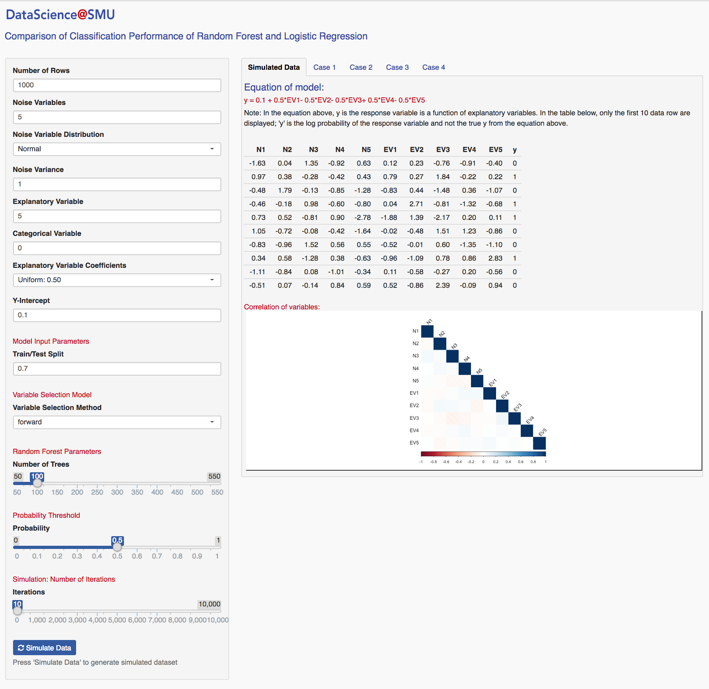
\includegraphics[width=0.8\textwidth]{rshiny.png}
\caption{R Shinny Application - Data Simulator}
\end{figure}


\section{Methods and Experiments}

The two machine learning algorithms studied in this work consist of random forest and logistic regression. Both models have been widely implemented in various disciplines for classification and regression purposes. Not only are these algorithms known for their success, but also their simplicity to implement and relatively straightforward to interpet. The functionality of Logistic Regression, a parameter based model, and random forest, a non-parametric model' are discussed in the following section. 

\subsection{Random Forest}


Random forest is an ensemble based learning algorithm which is comprised of 'n' collection of de-correlated decision trees (Hastie, 2009). Built off the idea of bootstrap aggregation which with a method for resampling with replacement in order to reduce variance, random forest uses multiple trees to average (regression) or compute majority votes (classification) in the terminal leaf nodes when making a prediction. Presented by Leo Breiman and built off the idea of decision trees, random forest models resulted significant improvements in prediction accuracy as compared to a single tree by growing 'n' number of trees where each tree in the training set is sampled randomly without replacement (Breiman ,1966). Decision trees consist simply of a tree-like structure where the top node is considered as the root of the tree and is recursively split at a series of decision nodes from the root until the terminal node or decision node is reached. 


\begin{figure}
\centering
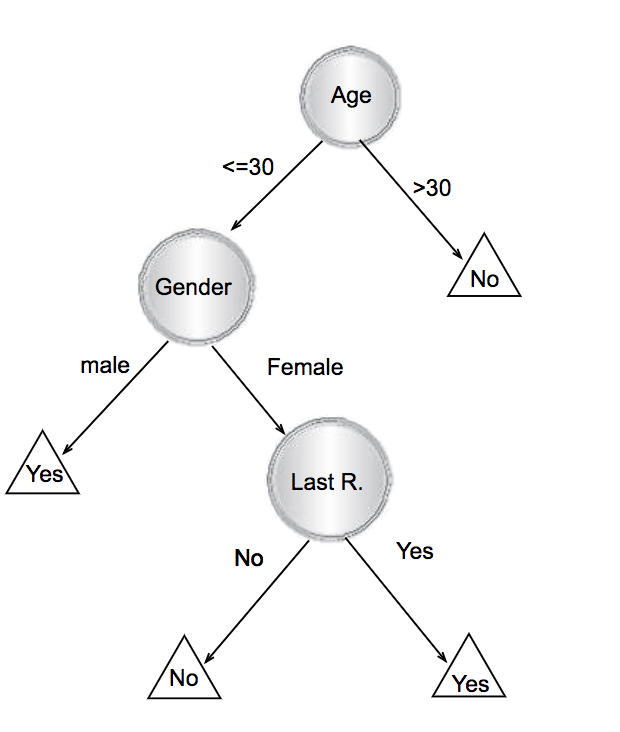
\includegraphics[width=0.5\textwidth]{decisiontree.png}
\caption{Example of Decision Tree (Lior Rokach et el)}
\end{figure}


As illustrated in the tree structure, the decision tree algorithm is a top down greedy approach by partitioning the dataset into smaller subsets; the result is a tree with a series of decision nodes and leaf node. The decision node has has two or more branches where the features with the highest information gain is split. The predictor variable that yields the highest informatio gain is the root node. The leaf node is represented as a prediction, and in this case, classifying either 1 or 0. Decision trees can handle both categorical and numerical data. First, in order to determine the information gain which is based on the entropy after splitting on an attribute, entropy is computed. Information gain is based on the principles from informaiton theory that uses entropy to compute impurity of datasets. Entropy measures the homogeneity of the subset data; if entropy equals one then the class labels are equally divided while an entropy of zero means the sample is completely homogeneous. 


\begin{equation}
Entropy = -p\log_{2}(p) - q\log_{2}(q)
\end{equation}


Advantages of using tree like learning algorithms allow for training models on large datasets in addition to quantitative and qualitative input variables. Additionally, tree based models can be immune to redundant variables or variables with high correlation which may lead to overfitting in other learning algorithms. Trees have also very few parameters to tune for when training the model and performs relatively well with outliers or missing values in a dataset. However, trees are prone to poor prediction performance; decision trees themselves are prone to overfitting noise in a training set which ultimately leads to results with high variance. In other words, this means the model could accurately predict the same data it was trained on but may not possess the same performance on datasets without the similar patterns and variations in the training set. Even fully grown decision trees are notorious for overfitting and do not generalize well to unseen data; random forest solves the overfitting conundrum by using a combination or "ensemble" of decision trees where the values in the tree are a random, independent, sample. 


\begin{figure}
\centering
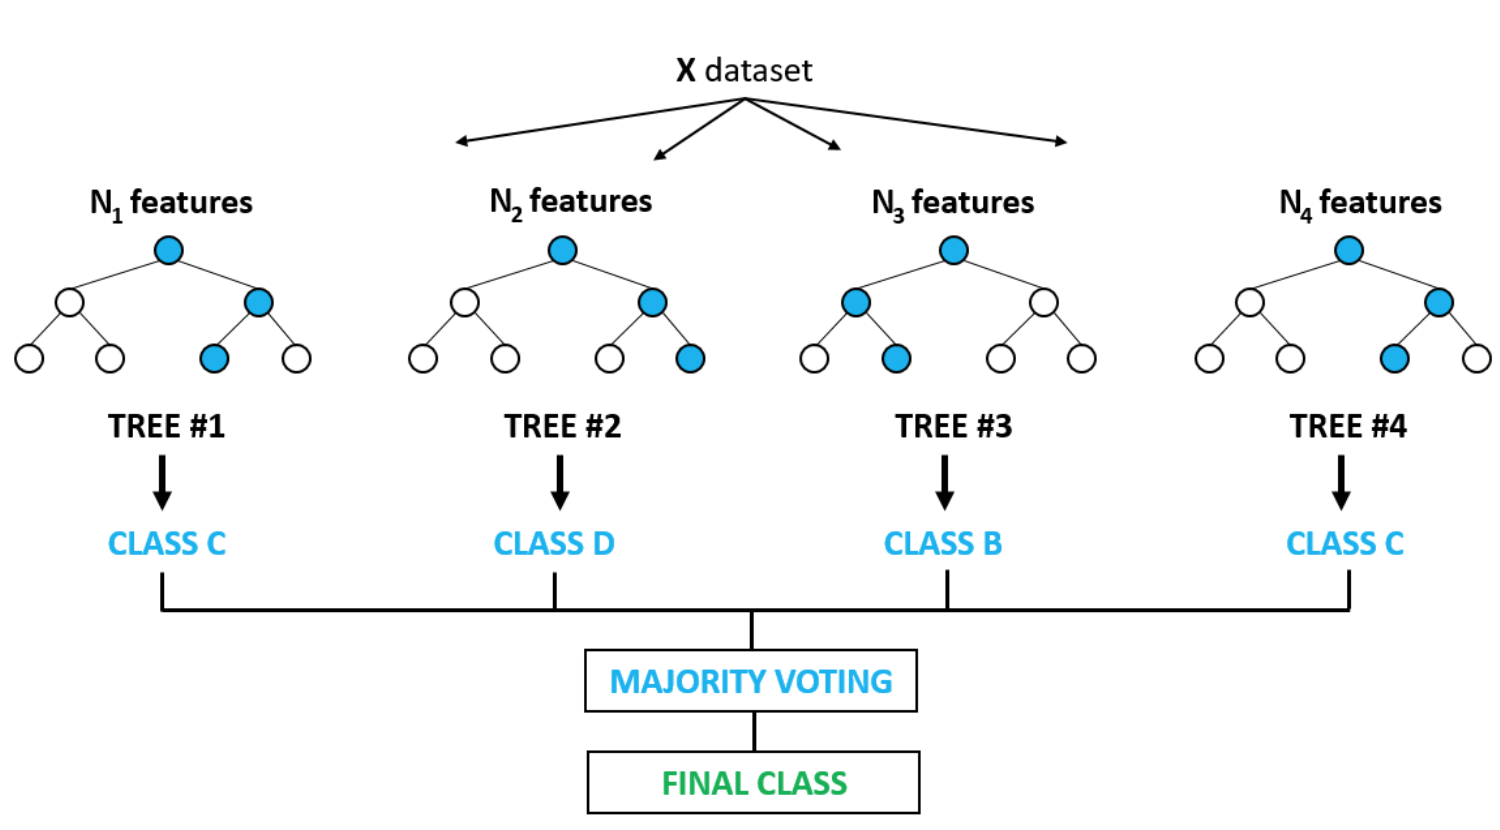
\includegraphics[width=0.90\textwidth]{randomforest.png}
\caption{Example of Decision Tree (Balazs Holczer)}
\end{figure}


The idea of randomly sampling the without replacement is known as bagging and this results in a different tree being generated to train on; averaging the results from the 'n' number of trees will result in decreasing the variance and establishing a smoother decision boundary (Hastie,  2009). For instance, while using random forest for classification, each tree will give an estimate of the probability of the class label, the probabilities will be averaged over the 'n' trees and the highest yields the predicted class label. In addition to bagging or bootstrap aggregation, in order to further reduces the variance in the decision boundary further, the trees must be completely uncorrelated and the method of bootstrapping alone is not enough. Breiman introduced the idea of randomly sampling 'm' number of features at each decision split in the tree as a way to decorrelate the trees in the random forest algorithm.  


\subsection{Logistic Regression}


Linear models are composed of one or multiple independent variables that describes a relationship to a dependent response variable. Mapping qualitative or quantitative input features to a target variable that is attempted to being predicted such as financial, biological, or sociological data is known as supervised learning in machine learning terminology if the labels are known.  One of the most common utilized linear statistical models for discriminant analysis is logistic Regression.

\begin{equation}
\pi_{i} = \beta_{0} + \beta_{1}X_{1} + .....\beta_{n}X_{n}
\end{equation}

Simplicity and interoperability of logistic Regression can occasionally lead to outperforming other sophisticated nonlinear models such as ensemble learners or support vector machines. However, in the event the response variable is drawn from a small sample size, then linear regression models become insufficient and performs poorly for binary responses A number of learning algorithms could be applied to modeling binary classification data types, however the focal point of this work is to examine one linear model, logistic regression. 
 
Unlike the response variable for Linear Regression which is quantitative, the target variable for logistic regression is the posterior probability of being classified in the ith group of a binary or multi-class response (Hastie, 2009). Logistic regression makes several assumptions such as independence, responses (logits) at every level of a subpopulation of the explanatory variable are normally distributed, and constant variance between the responses and all values of the explanatory variable. Intuitively, a transformation to the response variable is applied to yield a continuous probability distribution over the output classes bounded between 0 and 1; this transformation is called to “logistic” or “sigmoid” function where ‘z’ corresponds to log odds divided by the logit (Ng, 2008). The parameter estimates inform whether there is an increase or decrease in the predicted log odds of the response variable that would be predicted by one unit increase or decrease in one of the explanatory variables (e.g. x1), while holding all other explanatory variables constant.

\begin{equation}
\sigma(Z) = \frac{1}{1+\exp^{-z}}
\end{equation}


\begin{figure}
\centering
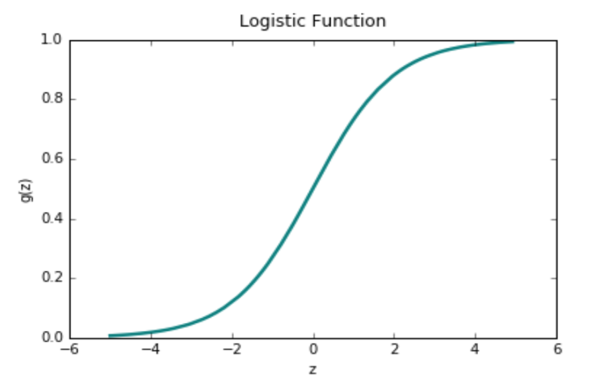
\includegraphics[scale=1.0]{sigmoid.png}
\caption{Logistic Function}
\end{figure}

For a binary response, the logistic regression model can be expressed by summing over the linear combinations of input features and a corresponding weight plus a bias terms for each instance as shown below in equation (3) and (4).

\begin{equation}
p(y^{(i)} = 1 | x^{(i)},w) = 1-  \frac{1}{1+\exp^{(w^{T}x^{(i)}+b)}}
\end{equation}
\begin{equation}
p(y^{(i)} = 0 | x^{(i)},w) = 1-  \frac{1}{1+\exp^{(w^{T}x^{(i)}+b)}}
\end{equation}


The objective is to find a set of weights such that the negative log likelihood is minimized over the defined training set using optimization techniques such as gradient descent or stochastic gradient descent [3]. Minimizing the negative log likelihood also means maximizing the likelihood or probability the parameter estimate pi of selecting the correct class. The loss function that measures the difference between the ground truth label and the predicted class label is referred to as the cross-entropy. If the prediction is very close to the ground truth label, the loss value will be low. Alternatively, if the prediction is far from the true label, the resulting log loss will be higher.

\begin{equation}
J(\theta) = -\frac{1}{m}\sum p_{i}log(y_{i}) + (1-p_{i})log(1-y_{i})
\end{equation}


\section{Analysis and Results}

\subsection{Case 1}

The first case investigated was comparing model performance with respect to change in variance in the explanatory and noise variables. The hypothesis was that an increase in variance would strengthen the accuracy for both models. For this simulation case, the application was configured to run 1000 simulations for 1000 observations. In Figure A, the results display the accuracy when there are 10 noise variables and 5 explanatory variables. The line graph shows that logistic regression looks to have a slightly higher accuracy over random forest.  However, to quantify this statistically, the p-value the paired two sample t-test was less than significance level of 0.05. In Figure B, the spread of accuracy for both models for all 1000 simulations is illustrated. From this plot, there is some overlap of the boxplots which suggests that although the line plots make linear regression look like a higher accuracy, random forest has very similar accuracy.

Figures C and D show the true positive rate and false positive rate respectively. The true positive rate for both models are nearly the same at each variance level.  However, one can see that the false positive rate for random forest is significantly higher than logistic regression (p-value = 0.63).  Even though both models have the same performance in terms of correctly classifying a true value as true, the false positive rate for random forest is higher than logistic regression.  This causes logistic regression to outperform random forest in terms of overall accuracy at each level of variance.

The simulation is then again, but now adding more noise variables (noise = 100) and the results of the accuracy is shown in Figure F. By looking at Figure A and Figure F, a similar trend is observed. With a p-value less than 0.05, there is no significant difference in accuracy between the two models. The boxplots for this simulation is also comparable to Figure B with 10 noise variables where minimal overlap in the boxplots for each model at each level of variance is observed. However, with 100 noise variables, the boxplots are much more consistent in that they are all about the same size for each level of variance.  In Figure B, the boxplots for each model are noticeably different sizes.

Figures I and J show the true positive rate and false positive rate respectively with 100 noise variables and 5 explanatory variables over increasing levels of variance in the variables. Interestingly, for variance 0.5 to 2.5 and a lot of noise, random forest has a higher true positive rate.  At around variance = 3.0 and higher, random forest still has a higher true positive rate, but it is not as large of a difference from logistic regression than variance < 2.5.  Unfortunately, as shown in Figure J the false positive rate for random forest is again higher than logistic regression so the gap in higher true positive rate is not enough to make overall accuracy higher for random forest.


\subsection{Case 2}

In the second simulation study, the model performance was evaluated with respect to change in the amount of noise in the dataset. Likewise, 1000 simulations were performed with the number of noise variables = 1, 5, 10, 20, 40, 60, 80, 100, 150, 200.  The results of the accuracy for each model when the number of explanatory variables is 5 with 1000 observations are shown in FigZ.  As expected, as the amount of noise in the dataset increases, the accuracy starts to decline for both models.

Figures C and D show the true positive rate and false positive rate respectively.  For true positive rate, when the number of noise variables is the less than or equal to the number of explanatory variables in the dataset, logistic regression is higher.  However, once the number of noise variables exceeds the number of explanatory variables, random forest begins to have a higher true positive rate than logistic regression.  As the amount of noise in the data increases, the false positive rate for both models also increases.  However, the rate of increase in false positive rate for random forest is greater than the rate of increase in false positive rate for logistic regression as noise increases. Furthermore, the simulations were tested with 10, 20 and 50 explanatory variables in the dataset and observed the same trends in model performance as with 5 explanatory variables.

\section{Ethics}

The disclaimer for utilizing this tool when selecting which machine learning model to implement in a production setting should done so with caution. Currently, the tool does not have certain functionalities to mimic real-world datasets, such as outliers or missing values to name a few. Failure to incorporate these types of characteristics in the simulated dataset can lead to inaccurate conclusions as to which algorithm yielded a better performance and thus any conclusions made from the RShiny tool may not generalize to these types of datasets. Moreover, the tool only considers random forest and logistic regression. As a result, other algorithms such as support vector machines or neural networks could produce higher prediciton accuracies and could be a better model to implement with datsets where the decision boundary is non-linearly seperable. Finally, in the context of the synthetic data generated in the application, there is no legal violations or security concerns. It should be clearly stated that the users should only consider the tool for educational purposes only as this application is still in the development phase. Any decisions drawn from the tool are not endorsed by the authors of this paper.


\section{Conclusions}



\section{Future Work}

The application provides the ability to answer in-depth statistical questions and evaluate classification perofrmance of two machine learning models, random forest and logistic regression. One of the objectives moving forward is to implement other algorithms such as Naive Bayes, XGBootst, and Artifical Neural Networks. Add more on hypyerparameter tuning, Grid Search, and applying k-fold cross-validation to further improvde model performance.....

\end{document}

